\section{Il modello scelto}
Per semplicità implementativa è stato scelto un modello preaddestrato. La scelta è ricaduta su Learning By Cheating(LBC) \cite{lbc}. LBC utilizza l'imitation learning come
approccio e divide la fase di addestramento in due fasi: \begin{itemize}
    \item nella prima viene addestrato un agente privilegiato sulla base di traiettorie di esperti. Questo agente ha accesso a tutte le informazioni 
    dell'ambiente circostante(layout ambientale, posizione di ogni altro partecipante). Agisce sull'ambiente con una vista dall'alto(birdview).
    \item nella seconda fase l'agente privilegiato fa da supervisore per l'addestramento di un agente sensorimotore. Questo ha accesso soltanto alle informazioni dei
    propri sensori(una camera RGB frontale). Viene addestrato per imitare l'agente privilegiato
\end{itemize}
L'apprendimento è stato suddiviso in due fasi per separare due compiti: imparare ad \emph{agire}, compito dell'agente privilegiato e imparare a \emph{vedere}, compito dell'agente sensorimotore.
Tale suddivisione porta i seguenti vantaggi:\begin{itemize}
    \item poichè l'agente privilegiato utilizza una rappresentazione compatta dell'ambiente, apprende più velocemente e generalizza meglio
    \item la supervisione fornita dall'agente privilegiato è di gran lunga più forte rispetto alle traiettorie originali, perchè può essere interrogato 
    su qualsiasi stato dell'ambiente
    \item l'agente privilegiato è di tipo white box e il suo stato interno può essere analizzato in qualsiasi istante
\end{itemize}
Nella figura \ref{fig:arch} è mostrata l'architettura dei due agenti. Concentrandosi sull'agente sensorimotore i casi l'input viene passato a una rete convoluzionale che produce una serie di 
waypoints nella camera frontale. Gli waypoints  sono selezionati sulla base del comando scelto e vengono passati al controllore di basso livello che produce un valore di sterzata, accelerazione o freno
\begin{figure}[h!]
    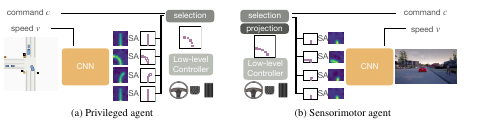
\includegraphics[width=\linewidth]{agenti.png}
    \caption{architettura dei due agenti\cite{lbc}}
    \label{fig:arch}
\end{figure}
